\section{Реализация}

Существует множество алгоритмов сборки мусора, однако одним из наиболее популярных является алгоритм пометки и освобождения
(англ. mark-and-sweep) и его вариации. Популярность данного алгоритма связана с минимальным количеством ограничений,
накладываемых на язык и сборщик мусора, и простотой самого алгоритма. Всё, что необходимо для его реализация ---
возможность построить корневое множество, уметь идентифицировать ссылки внутри объекта и иметь возможность
каким бы то ни было способом помечать объекты как живые. Данный алгоритм используется и во многих консервативных
сборщиках мусора, просто в таких случаях реализуемый сборщик мусора не является точным.
В классической реализации алгоритм пометки и освобождения является алгоритмом \textit{с полной остановкой мира}
(англ. stop-the-world),
иными словами, пользовательская программа прерывается на время работы сборщика мусора и продолжается после её окончания.
В предлагаемой работе будет использоваться именно вышеуказанный алгоритм. На то есть две основные причины:
во-первых, выбор конкретного алгоритма сборки мусора не является самоцелью данной работы,
во-вторых, предлагаемая реализация библиотеки сборки мусора предусматривает возможность дальнейшей реализации
широкого множества алгоритмов сборки мусора, как сжимающих или перемещающих, так и сборщиков мусора с
поколениями~\cite{GCHandbook}.

Как уже упоминалось ранее, используемый алгоритм сборки мусора делится на три фазы: построение корневого множества,
маркировку живых объектов, освобождение памяти. Реализация каждой фазы сборки мусора преставляет собой
ряд нижеописанных задач, подробное решение каждой из которых будет приведено в соответствующей части данной работы.

Для построения корневого множества необходимо решить, каким образом будет это корневое множество формироваться:
автоматически во время исполнения программы или же путем сканирования памяти
во время работы самого сборщика мусора, а также где и в каком виде хранить сами корни.
Для поиска корневых объектов нет необходимости сканировать всю память программы, достаточно ограничиться
программным стеком, регистрами и статической областью памяти~\cite{myCoursePaper}.
Для маркировки объекта необходимо иметь хотя бы один свободный бит в его заголовке или реализовывать некую структуру,
хранящую информацию о марке каждого объекта. Последнее решение является чрезмерно неэффективным по памяти, поэтому,
как правило, не используется. Существует несколько известных алгоритмов маркировки объектов:
\begin{enumerate}
\item \textit{Однобитная маркировка}. Выставляется один бит маркировки в заголовке объекта.
\item \textit{Трехцветная маркировка}. Выставляется два бита в заголовке объекта, говорящих о "цвете" объекта:
	\begin{enumerate}
	\item Белый. Означает, что объект ещё не был помечен. Изначально все объекты, кроме корней, белые.
	\item Серый. Означает, что объект уже помечен, но некоторые ссылки из него ещё не помечены. Корневое множество
		изначально серого цвета.
	\item Чёрный. Объект помечен, из него не осталось ссылок на белые объекты.
	\end{enumerate}
Существует несколько вариаций алгоритма трёхцветной маркировки, все они используются
исключительно для осуществления \textit{корнкурентной} маркировки объектов, т.е. маркировки объектов одновременно
с исполнением самой программы. Конкурентная маркировка используется для минимизации stop-the-world паузы.
\end{enumerate}
В реализумом сборщике мусора используется однобитная маркировка.
Реализация трехцветной маркировки является одним из возможных путей дальнейшего улучшения библиотеки.
Дополнительные биты в заголовке объекта появляются ввиду подмены стандартной кучи, используемой стандартным
\lstinline[language= cpp]{malloc} и \lstinline[language= cpp]{new}, на кучу Дага Ли.

\subsubsection{Malloc Дага Ли и его использование в сборщике мусора}
Malloc Дага Ли (Doug Lea's Malloc)\footnote{\cd{ftp://g.oswego.edu/pub/misc/malloc.c}}
представляет собой реализацию кучи, на основе которой
написан ptmalloc, используемый в библиотеке glib (GNU C library). Память кучи распределяется по сегментам (chunks), имеющим
восьмибайтовое выравнивание, содержащим заголовок и свободную память. Каждый блок памяти имеет свою метаинформацию в размере
8 или 16 байт, содержащую флаги, размер блока и указатели на предыдущий и последующий элементы (boundary tags),
сами же сегменты связаны по их размеру.

\begin{figure}[h!]
	\centering
	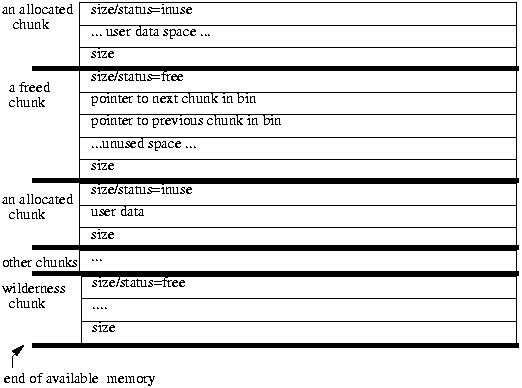
\includegraphics[width=300pt]{boundaryTags}
	\caption{Boundary Tags}
	\centering
	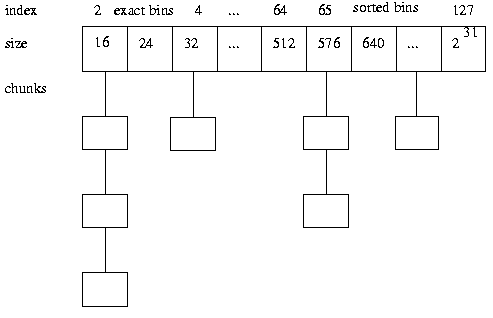
\includegraphics[width=300pt]{binding}
	\caption{Binding}
\end{figure}

Куча Дага Ли позволяет эффективно решать задачу освобождения неиспользуемой памяти.
Очевидно, что освобождение памяти извне программной кучи требует хранение дополнительной иформации о блоках памяти,
ставших мусором, и нетривиальную реализацию обхода этих блоков с целью освобождения, время которого будет весьма
чувствительно к внутреннему устройству кучи и алгоритмам освобождения памяти в ней.
Сама же куча могла бы сделать массовое освобождение памяти, а именно такое освобождение памяти происходит при сборке мусора,
куда более рационально, используя различные алгоритмы~\cite{GCBook}
и руководствуясь стратегией(-ями), которой данная реализация кучи придерживается.
Куча может вообще отложить часть работы по освобождению памяти до более подходящего времени,
исходя из принципа минимизации stop-the-world-паузы.
К счастью, существует модификация кучи Дага Ли,
предоставляющая эффективную функцию массового освобождения памяти~\cite{msmalloc}.
Более того, и нижесказанное является одной из основных причин использования кучи Дага Ли,
\lstinline[language= cpp]{dlmalloc} имеет бит маркировки в заголовке каждого сегмента. Совместно с функцией массового освобождения
памяти \lstinline[language= cpp]{dlmalloc} представляет собой готовую инфраструктуру для реализации сборки мусора.

Для обеспечения возможности совмещения ручного и автоматического управления памятью и маркировки объектов
реализованному сборщику мусора необходимо иметь два свободных бита в заголовке каждого объекта:
один бит для маркировки объекта, второй --- для флага, говорящего, является объект
управляемым или "ручным".
Куча Дага Ли при сборке в 64-x битной
системе ввиду выравнивания в заголовке объекта остаётся дополнительный свободный бит, который можно использовать.
Т.о. при сборке кучи в 64-x битной системе в заголовке объекта образуется один свободный бит
и бит маркировки, т.е. два бита, как того и требовалось.
Использование 64-x битной системы в данном случае чрезвычайно важно,
поскольку в 32-х битной версии дополнительного свободного бита нет. В последнем случае остаётся возможность
обеспечить сборку мусора, но для совмещения ручного и автоматического управления памятью необходимо было бы прибегнуть к
иным решениям. Ввиду вышесказанного использование 64-x битной системы является одним из ограничений
использования реализуемой библиотеки сборки мусора.
Немного подробнее об использовании двух битов в заголовке объекта для маркировки и совмещения ручного и автоматического
управления памятью:
\begin{enumerate}
\item По умолчанию аллокатор выставляет значение обоих битов в 0. Значение 0 первого бита означает, что объект "ручной".
\item При использовании примитивов самой библиотеки сборки мусора (ф-ия \lstinline[language= cpp]{gc_new} для выделения памяти),
	значение первого бита меняется на 1, что означает, что объект является управляемым.
\item Второй бит является битом маркировки: 0 --- объект не помечен, 1 --- объект помечен --- для управляемых
	объектов и не имеет никакого значения для "ручных".
\end{enumerate}
Т.о. достигается возможность совмещения ручного и автоматического управления памятью.
Разумеется, возникает проблема наличия ссылок из ручных объектов на управляемые,
подробное описание возникшей задачи и её решение расположено в части.

\subsubsection{Функции mmap и munmap}
Для работы с памятью, используемой для реализации сборщика мусора, используются следующие функции, позволяющие
работать с памятью вне программной кучи и стека, что позволяет избежать сборки мусора в самом сборщике мусора:
\begin{enumerate}
\item \lstinline[language= cpp]{void *mmap (void *, size_t, int, int, int, off_t)}\footnote{\cd{http://man7.org/linux/man-pages/man2/mmap.2.html}}
	для выделения памяти.\\*Функция принимает в качестве аргументов (слева направо):
	\begin{enumerate}
	\item желаемый адрес начала участка отбраженной памяти, если 0 --- ядро само выберет адрес;
	\item количество байт, которое нужно отобразить в память;
	\item число, определяющее степень защищённости отображенного участка памяти (только чтение, только запись, исполнение, область
		недоступна);
	\item атрибуты области;
	\item дескриптор файла, который нужно отобразить;
	\item смещение отображенного участка от начала файла.
	\end{enumerate}
	и возвращает адрес начала участка отображаемой памяти или \lstinline[language= cpp]{MAP_FAILED} в случае неудачи.
\item \lstinline[language= cpp]{int munmap (void *addr, size_t length)} для освобождения памяти.
	Параметр addr является адресом начала области памяти, выделенной для отображения файла, т.е. значением, которое вернул системный вызов \lstinline[language= cpp]{mmap}, параметр length определяет ее длину и его значение должно совпадать со значением соответствующего параметра в системном вызове \lstinline[language= cpp]{mmap}. При нормальном завершении системный вызов возвращает значение 0, при возникновении ошибки --- значение -1.	
\end{enumerate}

\subsection{Общая архитектура библиотеки сборки мусора}
На пользовательском уровне существует два основных примитива библиотеки:
\begin{enumerate}
\item "Умный"" указатель \lstinline[language= cpp]{gc_ptr<class_name>}. Представляет собой "умный" указатель на объект типа
	\lstinline[language= cpp]{class_name}.
	Данный примитив предлагается как альтернатива для указателей языка, являющаяся основой для идентификации ссылок из
	обного объекта на другой и построения корневого множества.
\item Функция выделения памяти \sloppy\lstinline[language= cpp]{<constructor_argument_types, allocation_object_type> gc_new (constructor_arguments, array_count = 1)}. Данный примитив используется для выделения автоматически управляемой памяти под объект типа \lstinline[language= cpp]{allocation_object_type} с помощью вызова конструктора объекта, имеющего типы параметров такие же и следующие в том же порядке, что передаются функции в списке \lstinline[language= cpp]{constructor argument types};
	\lstinline[language= cpp]{constructor_arguments} --- соответствующие перечисленным типам значения;
	\lstinline[language= cpp]{array_count} --- количество элементов массива, при выделении массива объектов типа
	\lstinline[language= cpp]{allocation_object_type}, по умолчанию равно 1, что означает выделение одиночного объекта.
\end{enumerate}
При использовании вышеуказанных примитивов следующим образом: \lstinline[language= cpp]{gc_ptr} вместо указателей языка и
\lstinline[language= cpp]{gc_new} в качестве единственной функции выделения памяти --- утверждается,
что управление памятью является автоматическим, а сборка мусора --- точной.

Связь между объектами системы представлена на рисунке \ref{fig:systemArch}. Подробное описание каждого компонента системы предоставлено
ниже в соответствующих частях.
\begin{figure}[h!]
	\centering
	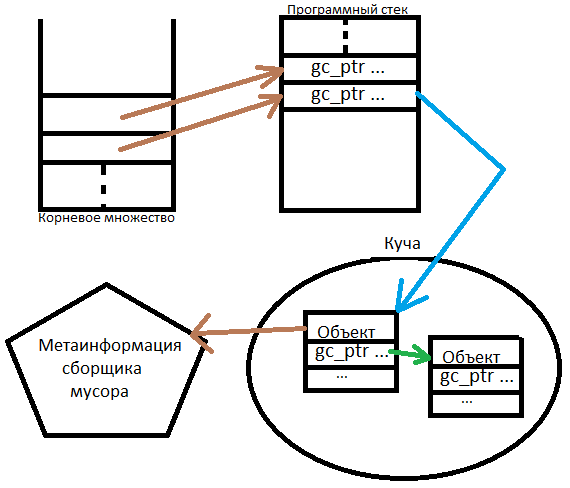
\includegraphics[width=250pt]{systemArch}
	\caption{Системные и пользовательские данные}
	\label{fig:systemArch}
\end{figure}

\subsection{Представление корней}
От того, каким образом хранятся корни, и насколько сложны операции поиска, удаления и добавления нового элемента,
напрямую зависит скорость выполнения фазы маркировки объектов и построения корневого множества.
В реализуемой библиотеке сборки мусора построение корневого множества происходит во время исполнения программы
следующим образом: при загрузке стековой рамки на стек все стековые объекты,
являющиеся \lstinline[language= cpp]{gc_ptr}, в своём конструкторе вызывают функцию добавления себя в корневое множество;
при вытеснении стековой рамки со стека эти же объекты вызывают функцию удаления себя из списка корневых объектов
в своём деструкторе; статические объекты, являющиеся \lstinline[language= cpp]{gc_ptr}, добавляются в корневое множество
в момент инициализации статической области и не удаляются оттуда в течение всего времени жизни программы.
Такой подход к построению корневого множества, разумеется, имеет свои минусы: при каждой загрузке/выгрузке
стековой рамки на/с вершину стека корневое множество будет меняться, образуя некоторую
задержку в исполнении программы. В случае, если между запусками сборки мусора есть значительное количество операций
над стеком, изменения корневого множества могут происходить впустую. Рис.\ref{fig:stackLive} иллюстрирует вышеизложенную мысль
на конкретном примере более наглядно: предположим, что между двумя соседними запусками сборки мусора было множество
операций загрузки/выгрузки стековых рамок, а сам стек остался таким же; корневое множество менялось при каждой такой
операции, но осталось при этом неизменным.

\begin{figure}[h!]
	\centering
	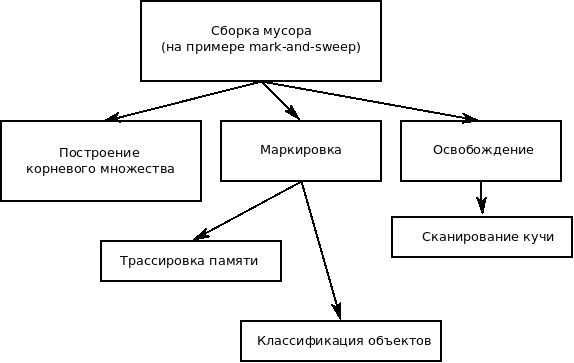
\includegraphics[width=250pt]{picture1}
	\caption{Пример стека при соседних запусках сборщика мусора}
	\label{fig:stackLive}
\end{figure}

Построение корневого множества исключительно в момент запуска самой сборки мусора
изменяло бы корневое множество лишь единожды, однако такое построение требует нетривиальной идентификации корней
в программном стеке, что может привести к долгосрочной паузе в исполнении программы, и не может являться
точным, поскольку невозможно в точности распознать все объекты определенного типа в программном стеке, не
внедряясь в компилятор, из-за возможности совпадения случайного значения в стеке с искомым объектом. Подобное
построение всегда консервативно.

Для решения задачи миниизации времени работы операций над корневым множество было предложено следующее решение:
\begin{enumerate}
\item Cтруктура для хранения корней представляет собой стек.
Согласно стандарту C++-11\footnote{\cd{https://isocpp.org/std/the-standard}} деструкторы стековых объектов вызываются в порядке, обратном вызову
их конструкторов, поэтому использование стека обусловлено быстротой выполнения операций вставки и удаления элементов.
Т.о. для удаления из корневого множества объекта достаточно произвести простой декремент указателя на вершину стека.
\item Стек представляет собой пул памяти.
Во избежание излишних затрат времени на маркировку самого корневого множества, которая вызывалась бы при каждом срабатывании
сборщика мусора, корневое множество реализовано не в программной куче, а в отдельном пуле памяти. Т.о. в фазе освобождения
памяти корневое множество не будет затронуто вовсе, а соответственно, и маркировка ему в таком случае не нужна,
что позволяет избежать хранения метаинформации для корневого множества, тем самым экономя память.
Сам же пул представляет собой динамическую область памяти, выделяемую с помощью функции \lstinline[language= cpp]{mmap}.
\item Стек реализован с использованием шаблона объектного проектирования singleton~\cite{patterns}.
Т.о. достигается уникальность корневого множества.
\end{enumerate} 

\subsection{Представление метаинформации}
Метаинформация в данной реализации сборщика мусора бывает двух типов: хранимая рядом с объектом и метаинформация для каждого класса, объект которого был хотя бы раз создан в куче.
Метаинформация, хранимая рядом с объектом, представляет собой простой указатель на метаинформацию класса,
которому данный объект принадлежит, и значение типа \lstinline[language= cpp]{size_t},
хранящего количество элементов массива, если объект представляет собой массив, 0 --- иначе.
Данный тип метаиформации расположен в памяти непосредственно перед самим объектом и имеет фиксированный размер.

\begin{figure}[h!]
	\centering
	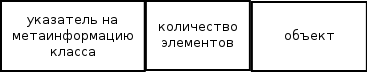
\includegraphics[width=250pt]{objectMeta}
	\caption{Метаинформация, хранимая рядом с объектом}
\end{figure}

Основной задачей, решаемой хранением метаинформации, является возможность обхода графа живых объектов на стадии маркировки,
начиная с корней. Происходит это следующим образом: по объекту находится метаинформация класса, которому он принадлежит;
в этой метаинформации хранятся смещения \lstinline[language= cpp]{gc_ptr} на другие объекты кучи относительно начала
самого объекта; функция маркировки запускается ото всех объектов, на которые ссылаются указатели,
лежащие на заданных смещениях от начала самого объекта.
Для поиска метаинформации класса, которому принадлежит объект, достаточно перейти по указателю, лежащему в метаинформации
объекта непосредственно перед ним.
Сама метаинфомация класса вычисляется в момент создания первого объекта подобного типа и заносится в список пар
<имя класса, его метаинформация>. Метаинформация класса представляет собой специальным образом хранимые смещения
указателей на другие элементы класса от начала объекта. У всех объектов одного типа смещения от начала объекта до его полей
неизменны, что и позволяет высчитать их для каждого класса лишь единожды.
Подробнее об этом процессе можно прочитать в работе~\cite{kren}.

Метаинформация класса бывает двух типов:
\begin{enumerate}
\item \lstinline[language= cpp]{box_simple} --- для простых объектов и массивов \textit{простых объектов},
	т.е. объектов, не содержащих ссылок в кучу. Представляет собой просто метку о том, что объект не содержит ссылок на другие
	объекты кучи.
\item \lstinline[language= cpp]{generic_box_struct} --- для объектов, имеющих ссылки в кучу внутри себя.
	В памяти подряд хранятся структуры, каждая из которых хранит смещение объекта до очередной ссылки из него и бит,
	говорящий о том, является ли данная ссылка ссылкой на простой объект или же нет.
\end{enumerate}
Структура для хранения метаинформации представляет собой список пар <указатель на имя класса, указатель на метаинформацию класса>,
для краткости далее будем называть этот список просто \textit{список метаинформации классов}.
Имена классов хранятся подряд в отдельном пуле памяти, вычисляются с помощью шаблонов C++ с использованием
функции \lstinline[language= cpp]{typeid} в момент выделения памяти под объект.
Подобное представление позволяет хранить исключительно имена классов без какой-либо дополнительной метаинформации о них
или реализации специальных структур данных, что, несомненно, экономит память программы.
Очевидно, что предложенная реализация затрудняет поиск элемента в пуле и его удаление, однако
операций поиска и удаления элементов из пула памяти с именами классов не происходит, потому что метаинформация,
будучи единожды созданной для класса, уже не удаляется, т.к. всегда может понадобиться в дальнейшем, соответственно
и имя класса также необходимо хранить. Поиск элемента в пуле для имен классов также не происходит,
поскольку для любого имени класса существует запись в списке метаинформации классов, в котором и происходит
поиск метаинформации класса при создании объекта с помощью функции \lstinline[language= cpp]{gc_new}.

\begin{figure}[h!]
	\centering
	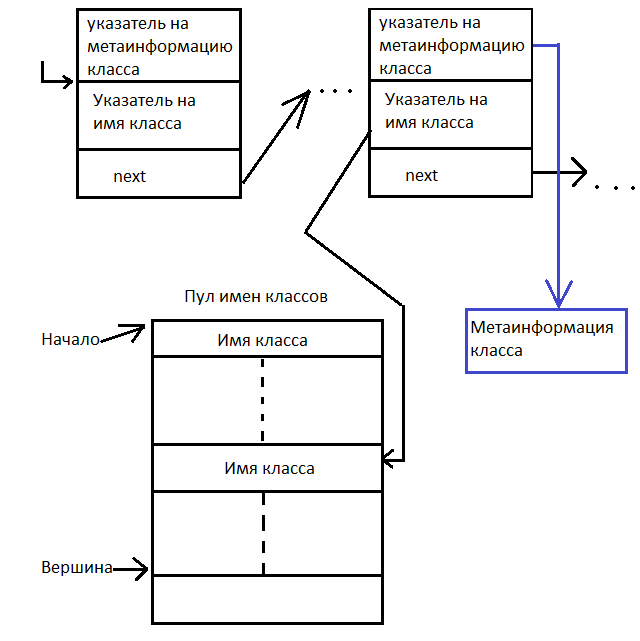
\includegraphics[width=350pt]{picture2}
	\caption{Представление метаинформации}
\end{figure}

\newpage
\subsection{Совмещение ручного и автоматического управления памятью}
Как уже говорилось, пользователю предоставляется возможность совмещения автоматического и ручного управления памятью,
в связи с чем возникает следующая проблема: наличие ссылки из ручного на управляемый объект.
В случае, если более не осталось ссылок из управляемых объектов на данный объект, а из ручного на него ссылка есть,
сборщик мусора удалит рассматриваемый объект, и ссылка станет висячей.
Предлагается следующее решение данной проблемы: предоставить пользователю функцию регистрации и дерегистрации управляемого объекта
как \textit{мнимого корня}, т.е. объекта, который приравнивается к корневым, хотя таковым не является.
Поскольку порядок регистрации и дерегистрации объекта, как мнимого корня, никак не определен и происходит исключительно по желанию пользователя, оптимизировать их хранение столь же эффективно, как хранение обычных корней, не представляется возможным,
в связи с чем все мнимые корни хранятся в отдельной древовидной структуре, хранимой в куче.

Конечно, такой подход небезопасен, поскольку, в случае ошибки пользователя, могут возникнуть висячие ссылки, или появиться несобираемый мусор, если пользователь забудет дерегистрировать объект.
Но, стоит заметить, что возникновение ошибок подобного рода никоим образом нельзя избежать при ручном управлении памятью.